\documentclass{article}
\usepackage[utf8]{inputenc}

\title{Design Document for Stickiero}
\author{Erik Andersson \and Daniel Backlund \and Mattias Linder \and Joel Wiklund \\\\Group 1\\Version 1.0}
\date{Mars 2015}

\usepackage{natbib}
\usepackage{graphicx}
\usepackage{hyperref}

\begin{document}

\maketitle
\clearpage

\begin{abstract}
  Abstract.
\end{abstract}
\tableofcontents

\subsection*{Changelog}
\addcontentsline{toc}{subsection}{Changelog}
\paragraph{}
\em{}Version 1.0:\em{} Created document.\\ 
\clearpage

\part{Design Overview}
\section{Personas}
\label{sec:label}
\subsection{Persona 1}

\textbf{Name}: Liam Svensson\\
\textbf{Age}: 10\\
\textbf{Computer knowledge}: Medium\\
\textbf{Gaming experience}: Medium, playing for 3 years\\
\textbf{Interests}: Gaming, dinosaurs and McDonalds\\\\
Likes playing all kinds of game. Has been playing since he was 7. 

\subsection{Persona 2}

\textbf{Name}: Anders Svensson\\
\textbf{Age}: 15\\
\textbf{Computer knowledge}: Medium\\
\textbf{Gaming experience}: High, playing for 7 years\\
\textbf{Interests}: Gaming and watch streams on twitch.com\\\\
Anders is a hardcore gamer and he likes games that requires more skills. He is competitive in his gaming and wants to perform good when playing.

\subsection{Persona 3}

\textbf{Name}: Anna Svensson\\
\textbf{Age}: 43\\
\textbf{Computer knowledge}: Low\\
\textbf{Gaming experience}: Low\\
\textbf{Interests}: Design and travels\\\\
Like Danish design and loves to travel abbroad. Has not played many games except some games on her phone. 

\newpage
\section{Scenarios}
\label{sec:label}
\subsection{Persona 1}
Liam wants to play a new game that his friend has told him about. It is called Stickiero. He downloads the demo on his computer and starts playing. He found the controls pretty easy to understand since he has used keyboard and mouse before. His mom walks in on him and sees him playing Stickero. She is horrified by the amount of blood displayed on the screen. She tells Liam to stop playing this horrible game and go to his room.
\subsection{Persona 2}
Anders is Liams older brother. He heard the fight between Liam and his mother about some game being brutal. He downloads this game on his own computer and tries it out. He has played the original game Liero before. He finds that the graphic is better and the amount of blood satisfies him. But the controls are made too easy he thinks. It is too easy to aim and hit the other player. He feels like there should be a mode where you can have the original controls.
\subsection{Persona 3}
Anna is Liams and Anders mother. She decides to try the game out so she can decide if Liams should be allowed to play the game. She founds it very violent, especially with all the blood. But she found there is a parental version of the game on the Internet which does not contain any blood. She decides that Liam will be playing the parental version of the game. She does not find the gamy specially fun to play since she could not figure out how to play the game. She feels like there should have been a tutorial that explains how to play the game and what to do in the game.

\newpage
\section{Requirements specification}

\begin{tabular}{ | c | r |}
  \hline                       
   \textbf{Functional} & \textbf{Non-functional} \\
   Able to rebind key bindings & Any alphabetic character \\
   Change screen size and resolution & Some max/min screen size \\
   Volume control & Mute/unmute\\
   Parental version & Green blood and more friendly sound\\
   Aim with either mouse or keyboard & None \\
   Local multiplayer, see below for screen handling  & 2 players \\
   Choose Split screen or zoom & Vertical split, max/min zoom \\
   Change weapons & None \\
   Change skins & None \\
   Game mode & Deathmatch, capture the flag etc... \\
   Max time per match & max time 60 min min time 1 min\\
   Multiplayer over net & 2 to 4 players \\
   Customize name & Max characters 10 \\
   Tutorial & One tutorial level \\
   Undo/Redo & At settings screen \\
   Internatinalization & English and swedish \\
   Sound effects & Jumping, shooting, death etc...\\
  \hline  
\end{tabular}

\clearpage
\section{Scrum plan}
\begin{figure}[h!]
\centering
\frame{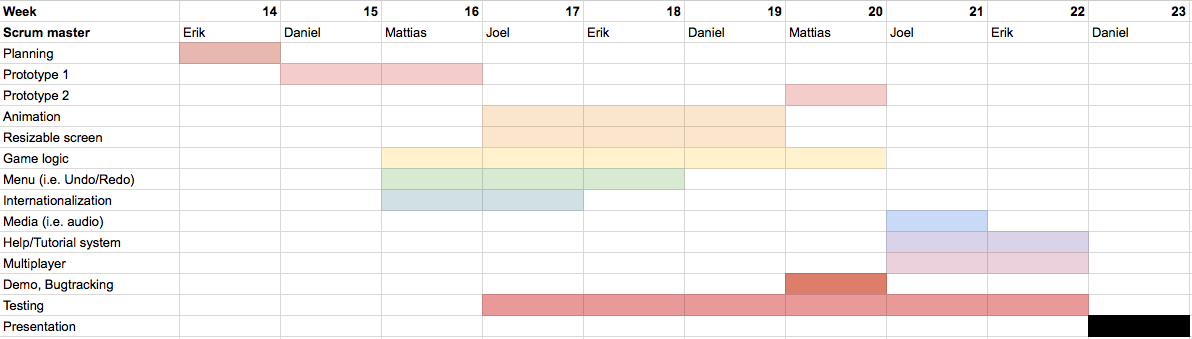
\includegraphics[width=\textwidth, height=\textheight, keepaspectratio, natwidth=720, natheight=540]{scrumplan.png}}
\caption{First Scrum plan}
\label{fig:scrumplan}
\end{figure}

\clearpage
\section{UML}
\begin{figure}[h!]
\centering
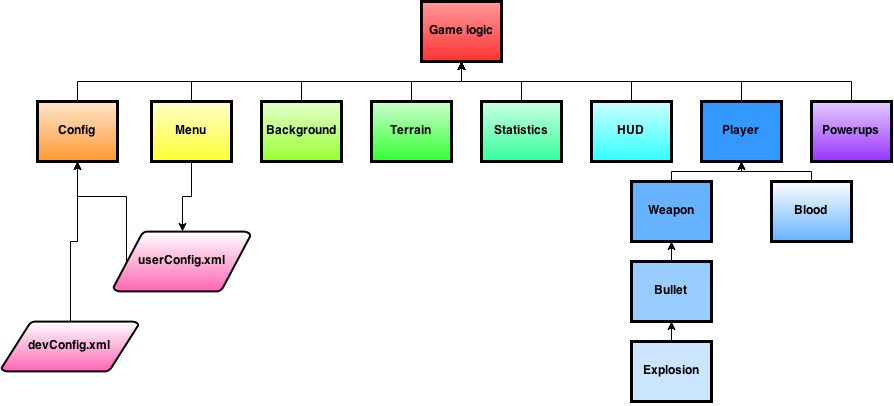
\includegraphics[width=\textwidth, height=\textheight, keepaspectratio, natwidth=720, natheight=540]{uml.png}
\caption{UML}
\label{fig:uml}
\end{figure}
\clearpage
\section{Comments on project requirements}
The project will make a clone of the old school game Liero. In the game you are a worm which is supposed to kill an enemy worm.
\\ \\
\textbf{Must include...} \\
\textbf{...an animated, interactive part}
\\ - The worms and weapons will be animated. \\
\textbf{...a resizable screen}
\\ - The graphics will be in different resolutions making it easy to resize the screen. \\
\textbf{...interaction with graphics}
\\ - The terrain will be destructible. \\
\textbf{...an interactive help/tutorial system}
\\ - The game will have different maps, where one is a tutorial map. \\
\textbf{...at least one media file (sound, video, etc.)}
\\ - The weapons will have sound effects and the worms will make sounds. \\
(See Figure~\ref{fig:liero})
\\ \\
\textbf{...multi/bilingual interface} \\
 - The settings and the HUD are LN18. \\
\textbf{...undo/redo (when feasible)} \\
 - The settings page is undoable/redoable. \\
(See Figure~\ref{fig:liero2})


\begin{figure}[h!]
\centering
\frame{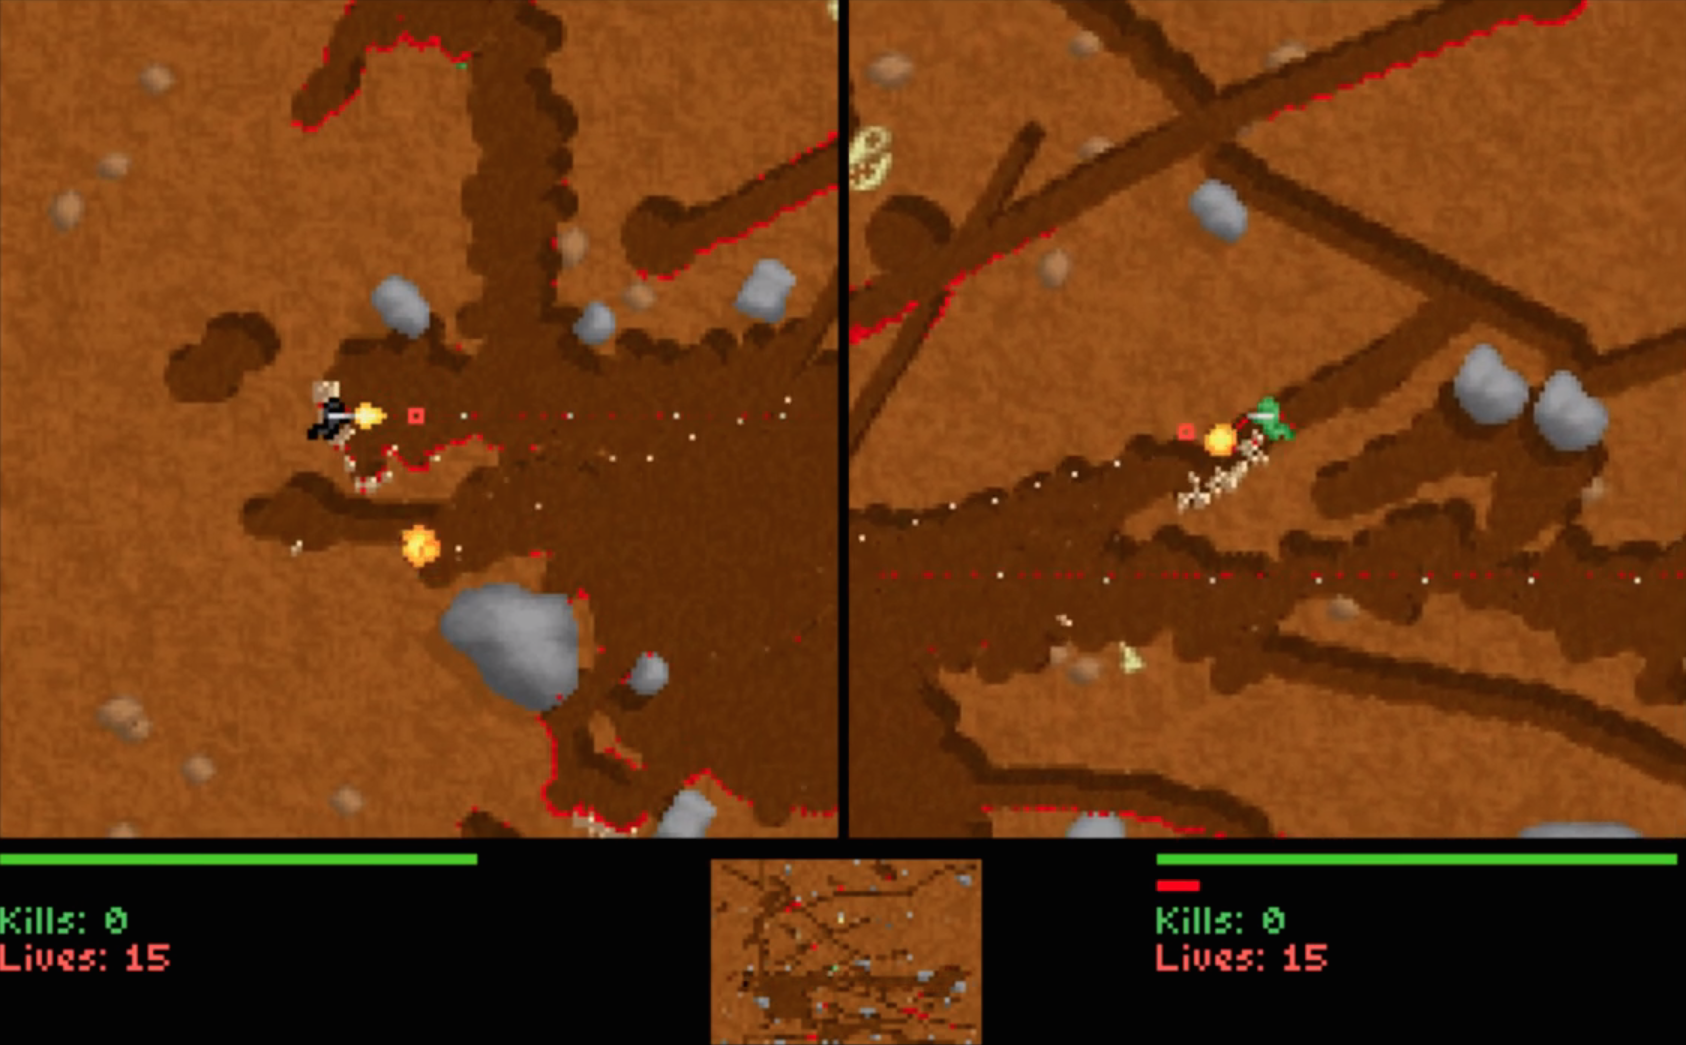
\includegraphics[width=\textwidth, height=\textheight, keepaspectratio, natwidth=720, natheight=540]{screen1.png}}
\caption{Screenshot from original Liero}
\label{fig:liero}
\end{figure}

\begin{figure}[h!]
\centering
\frame{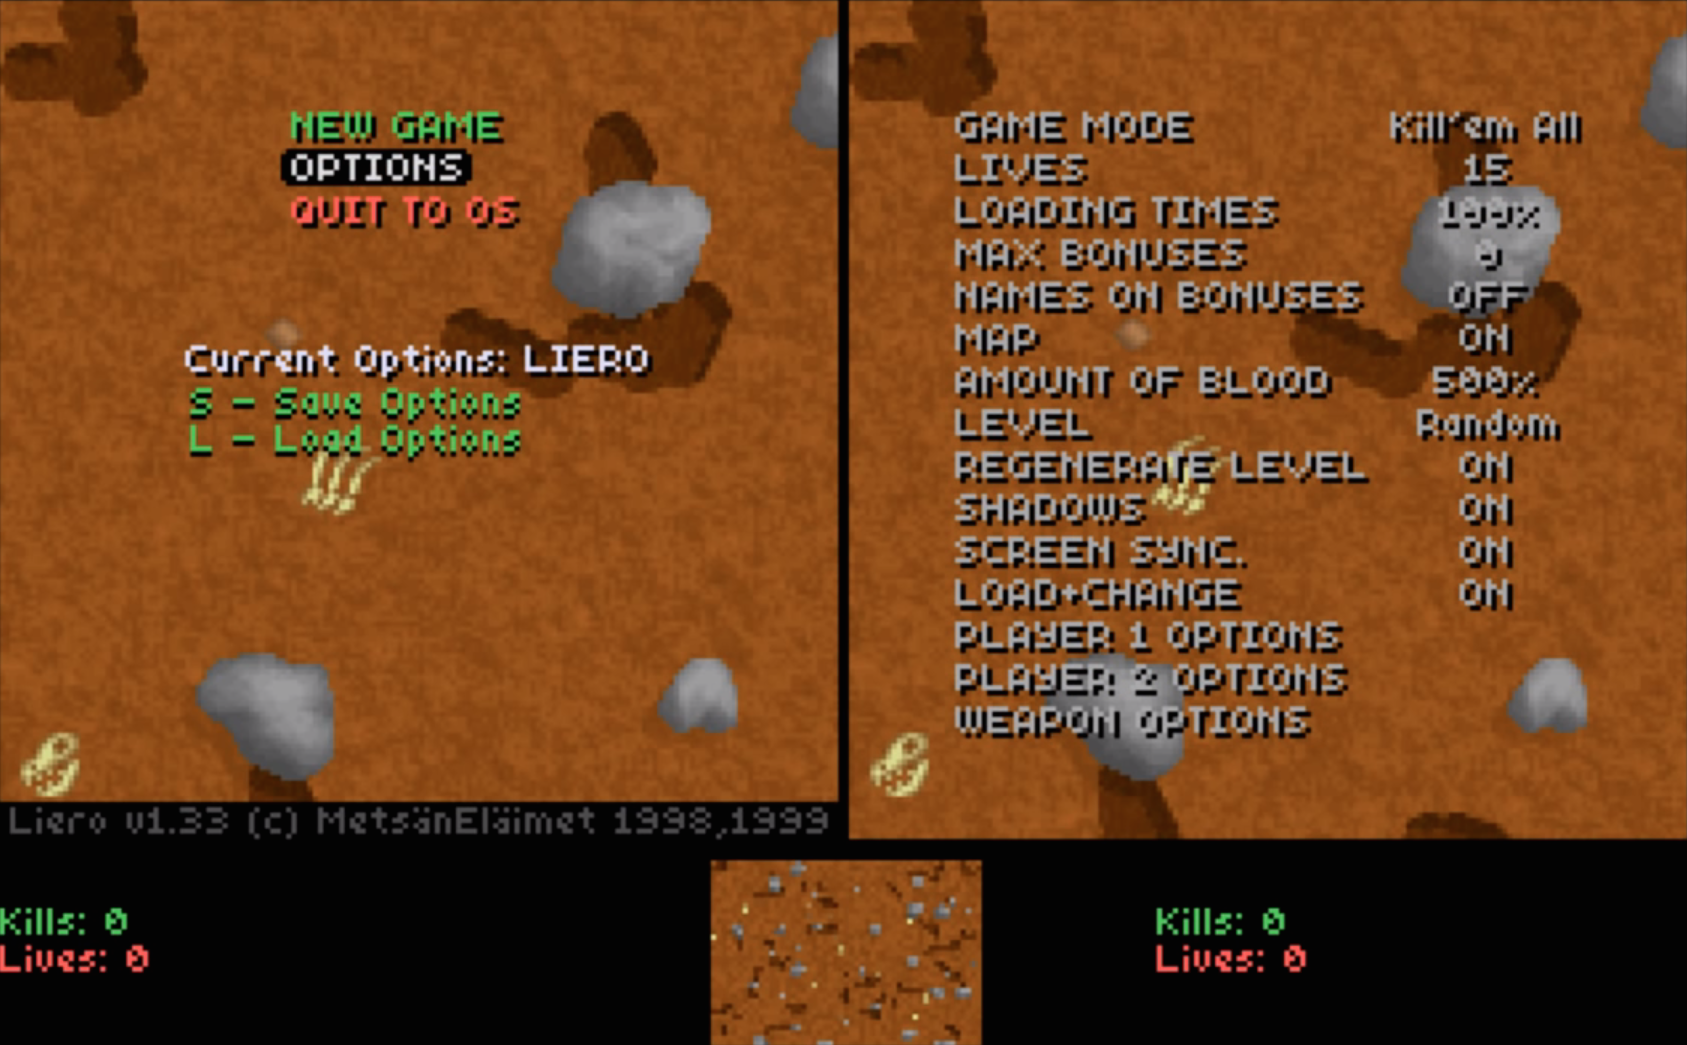
\includegraphics[width=\textwidth, height=\textheight, keepaspectratio, natwidth=720, natheight=540]{screen2.png}}
\caption{Screenshot from original Liero}
\label{fig:liero2}
\end{figure}

\clearpage
\end{document}
